% Created by tikzDevice version 0.8.1 on 2015-11-17 11:43:47
% !TEX encoding = UTF-8 Unicode
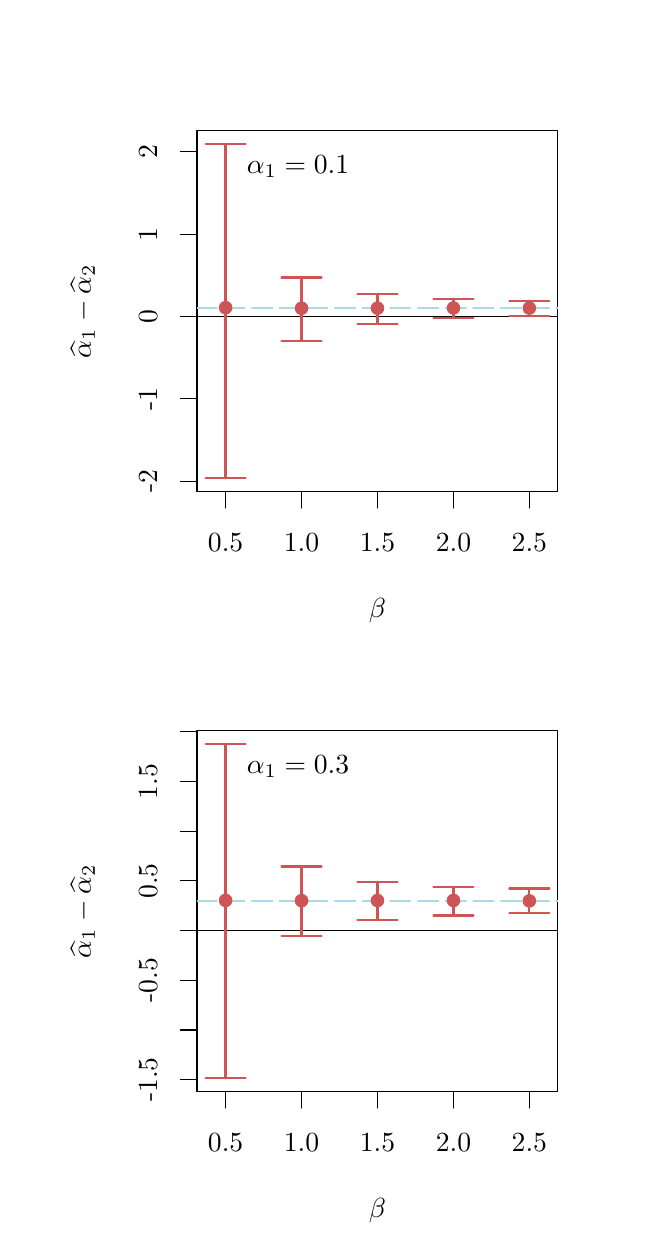
\begin{tikzpicture}[x=1pt,y=1pt]
\definecolor{fillColor}{RGB}{255,255,255}
\path[use as bounding box,fill=fillColor,fill opacity=0.00] (0,0) rectangle (216.81,433.62);
\begin{scope}
\path[clip] ( 61.20,266.01) rectangle (191.61,396.42);
\definecolor{drawColor}{RGB}{255,255,255}
\definecolor{fillColor}{RGB}{255,255,255}

\path[draw=drawColor,line width= 0.4pt,line join=round,line cap=round,fill=fillColor] ( 71.52,332.44) circle (  2.25);

\path[draw=drawColor,line width= 0.4pt,line join=round,line cap=round,fill=fillColor] ( 98.96,332.22) circle (  2.25);

\path[draw=drawColor,line width= 0.4pt,line join=round,line cap=round,fill=fillColor] (126.40,332.26) circle (  2.25);

\path[draw=drawColor,line width= 0.4pt,line join=round,line cap=round,fill=fillColor] (153.85,332.32) circle (  2.25);

\path[draw=drawColor,line width= 0.4pt,line join=round,line cap=round,fill=fillColor] (181.29,332.28) circle (  2.25);
\end{scope}
\begin{scope}
\path[clip] (  0.00,  0.00) rectangle (216.81,433.62);
\definecolor{drawColor}{RGB}{0,0,0}

\path[draw=drawColor,line width= 0.4pt,line join=round,line cap=round] ( 71.52,266.01) -- (181.29,266.01);

\path[draw=drawColor,line width= 0.4pt,line join=round,line cap=round] ( 71.52,266.01) -- ( 71.52,260.01);

\path[draw=drawColor,line width= 0.4pt,line join=round,line cap=round] ( 98.96,266.01) -- ( 98.96,260.01);

\path[draw=drawColor,line width= 0.4pt,line join=round,line cap=round] (126.40,266.01) -- (126.40,260.01);

\path[draw=drawColor,line width= 0.4pt,line join=round,line cap=round] (153.85,266.01) -- (153.85,260.01);

\path[draw=drawColor,line width= 0.4pt,line join=round,line cap=round] (181.29,266.01) -- (181.29,260.01);

\node[text=drawColor,anchor=base,inner sep=0pt, outer sep=0pt, scale=  1.00] at ( 71.52,244.41) {0.5};

\node[text=drawColor,anchor=base,inner sep=0pt, outer sep=0pt, scale=  1.00] at ( 98.96,244.41) {1.0};

\node[text=drawColor,anchor=base,inner sep=0pt, outer sep=0pt, scale=  1.00] at (126.40,244.41) {1.5};

\node[text=drawColor,anchor=base,inner sep=0pt, outer sep=0pt, scale=  1.00] at (153.85,244.41) {2.0};

\node[text=drawColor,anchor=base,inner sep=0pt, outer sep=0pt, scale=  1.00] at (181.29,244.41) {2.5};

\path[draw=drawColor,line width= 0.4pt,line join=round,line cap=round] ( 61.20,269.76) -- ( 61.20,388.78);

\path[draw=drawColor,line width= 0.4pt,line join=round,line cap=round] ( 61.20,269.76) -- ( 55.20,269.76);

\path[draw=drawColor,line width= 0.4pt,line join=round,line cap=round] ( 61.20,299.52) -- ( 55.20,299.52);

\path[draw=drawColor,line width= 0.4pt,line join=round,line cap=round] ( 61.20,329.27) -- ( 55.20,329.27);

\path[draw=drawColor,line width= 0.4pt,line join=round,line cap=round] ( 61.20,359.03) -- ( 55.20,359.03);

\path[draw=drawColor,line width= 0.4pt,line join=round,line cap=round] ( 61.20,388.78) -- ( 55.20,388.78);

\node[text=drawColor,rotate= 90.00,anchor=base,inner sep=0pt, outer sep=0pt, scale=  1.00] at ( 46.80,269.76) {-2};

\node[text=drawColor,rotate= 90.00,anchor=base,inner sep=0pt, outer sep=0pt, scale=  1.00] at ( 46.80,299.52) {-1};

\node[text=drawColor,rotate= 90.00,anchor=base,inner sep=0pt, outer sep=0pt, scale=  1.00] at ( 46.80,329.27) {0};

\node[text=drawColor,rotate= 90.00,anchor=base,inner sep=0pt, outer sep=0pt, scale=  1.00] at ( 46.80,359.03) {1};

\node[text=drawColor,rotate= 90.00,anchor=base,inner sep=0pt, outer sep=0pt, scale=  1.00] at ( 46.80,388.78) {2};

\path[draw=drawColor,line width= 0.4pt,line join=round,line cap=round] ( 61.20,266.01) --
	(191.61,266.01) --
	(191.61,396.42) --
	( 61.20,396.42) --
	( 61.20,266.01);
\end{scope}
\begin{scope}
\path[clip] (  0.00,216.81) rectangle (216.81,433.62);
\definecolor{drawColor}{RGB}{0,0,0}

\node[text=drawColor,anchor=base,inner sep=0pt, outer sep=0pt, scale=  1.00] at (126.41,220.41) {$\beta$};

\node[text=drawColor,rotate= 90.00,anchor=base,inner sep=0pt, outer sep=0pt, scale=  1.00] at ( 22.80,331.22) {$\widehat{\alpha}_1 - \widehat{\alpha}_2$};
\end{scope}
\begin{scope}
\path[clip] ( 61.20,266.01) rectangle (191.61,396.42);
\definecolor{drawColor}{RGB}{0,0,0}

\node[text=drawColor,anchor=base west,inner sep=0pt, outer sep=0pt, scale=  1.00] at ( 79.20,380.98) {$\alpha_1=0.1$};
\definecolor{drawColor}{RGB}{173,216,230}

\path[draw=drawColor,line width= 0.8pt,dash pattern=on 7pt off 3pt ,line join=round,line cap=round] ( 61.20,332.25) -- (191.61,332.25);

\path[draw=drawColor,line width= 0.8pt,dash pattern=on 7pt off 3pt ,line join=round,line cap=round] ( 61.20,332.25) -- (191.61,332.25);

\path[draw=drawColor,line width= 0.8pt,dash pattern=on 7pt off 3pt ,line join=round,line cap=round] ( 61.20,332.25) -- (191.61,332.25);

\path[draw=drawColor,line width= 0.8pt,dash pattern=on 7pt off 3pt ,line join=round,line cap=round] ( 61.20,332.25) -- (191.61,332.25);

\path[draw=drawColor,line width= 0.8pt,dash pattern=on 7pt off 3pt ,line join=round,line cap=round] ( 61.20,332.25) -- (191.61,332.25);
\definecolor{drawColor}{RGB}{0,0,0}

\path[draw=drawColor,line width= 0.4pt,line join=round,line cap=round] ( 61.20,329.27) -- (191.61,329.27);
\definecolor{drawColor}{RGB}{205,85,85}

\path[draw=drawColor,line width= 0.8pt,line join=round,line cap=round] ( 71.52,270.84) -- ( 71.52,391.59);

\path[draw=drawColor,line width= 0.8pt,line join=round,line cap=round] ( 64.29,270.84) --
	( 71.52,270.84) --
	( 78.75,270.84);

\path[draw=drawColor,line width= 0.8pt,line join=round,line cap=round] ( 78.75,391.59) --
	( 71.52,391.59) --
	( 64.29,391.59);

\path[draw=drawColor,line width= 0.8pt,line join=round,line cap=round] ( 98.96,320.47) -- ( 98.96,343.36);

\path[draw=drawColor,line width= 0.8pt,line join=round,line cap=round] ( 91.73,320.47) --
	( 98.96,320.47) --
	(106.19,320.47);

\path[draw=drawColor,line width= 0.8pt,line join=round,line cap=round] (106.19,343.36) --
	( 98.96,343.36) --
	( 91.73,343.36);

\path[draw=drawColor,line width= 0.8pt,line join=round,line cap=round] (126.40,326.60) -- (126.40,337.37);

\path[draw=drawColor,line width= 0.8pt,line join=round,line cap=round] (119.18,326.60) --
	(126.40,326.60) --
	(133.63,326.60);

\path[draw=drawColor,line width= 0.8pt,line join=round,line cap=round] (133.63,337.37) --
	(126.40,337.37) --
	(119.18,337.37);

\path[draw=drawColor,line width= 0.8pt,line join=round,line cap=round] (153.85,328.71) -- (153.85,335.69);

\path[draw=drawColor,line width= 0.8pt,line join=round,line cap=round] (146.62,328.71) --
	(153.85,328.71) --
	(161.08,328.71);

\path[draw=drawColor,line width= 0.8pt,line join=round,line cap=round] (161.08,335.69) --
	(153.85,335.69) --
	(146.62,335.69);

\path[draw=drawColor,line width= 0.8pt,line join=round,line cap=round] (181.29,329.52) -- (181.29,334.96);

\path[draw=drawColor,line width= 0.8pt,line join=round,line cap=round] (174.06,329.52) --
	(181.29,329.52) --
	(188.52,329.52);

\path[draw=drawColor,line width= 0.8pt,line join=round,line cap=round] (188.52,334.96) --
	(181.29,334.96) --
	(174.06,334.96);
\definecolor{fillColor}{RGB}{205,85,85}

\path[draw=drawColor,line width= 0.4pt,line join=round,line cap=round,fill=fillColor] ( 71.52,332.44) circle (  2.25);

\path[draw=drawColor,line width= 0.4pt,line join=round,line cap=round,fill=fillColor] ( 98.96,332.22) circle (  2.25);

\path[draw=drawColor,line width= 0.4pt,line join=round,line cap=round,fill=fillColor] (126.40,332.26) circle (  2.25);

\path[draw=drawColor,line width= 0.4pt,line join=round,line cap=round,fill=fillColor] (153.85,332.32) circle (  2.25);

\path[draw=drawColor,line width= 0.4pt,line join=round,line cap=round,fill=fillColor] (181.29,332.28) circle (  2.25);
\end{scope}
\begin{scope}
\path[clip] ( 61.20, 49.20) rectangle (191.61,179.61);
\definecolor{drawColor}{RGB}{255,255,255}
\definecolor{fillColor}{RGB}{255,255,255}

\path[draw=drawColor,line width= 0.4pt,line join=round,line cap=round,fill=fillColor] ( 71.52,118.25) circle (  2.25);

\path[draw=drawColor,line width= 0.4pt,line join=round,line cap=round,fill=fillColor] ( 98.96,118.17) circle (  2.25);

\path[draw=drawColor,line width= 0.4pt,line join=round,line cap=round,fill=fillColor] (126.40,118.22) circle (  2.25);

\path[draw=drawColor,line width= 0.4pt,line join=round,line cap=round,fill=fillColor] (153.85,118.24) circle (  2.25);

\path[draw=drawColor,line width= 0.4pt,line join=round,line cap=round,fill=fillColor] (181.29,118.09) circle (  2.25);
\end{scope}
\begin{scope}
\path[clip] (  0.00,  0.00) rectangle (216.81,433.62);
\definecolor{drawColor}{RGB}{0,0,0}

\path[draw=drawColor,line width= 0.4pt,line join=round,line cap=round] ( 71.52, 49.20) -- (181.29, 49.20);

\path[draw=drawColor,line width= 0.4pt,line join=round,line cap=round] ( 71.52, 49.20) -- ( 71.52, 43.20);

\path[draw=drawColor,line width= 0.4pt,line join=round,line cap=round] ( 98.96, 49.20) -- ( 98.96, 43.20);

\path[draw=drawColor,line width= 0.4pt,line join=round,line cap=round] (126.40, 49.20) -- (126.40, 43.20);

\path[draw=drawColor,line width= 0.4pt,line join=round,line cap=round] (153.85, 49.20) -- (153.85, 43.20);

\path[draw=drawColor,line width= 0.4pt,line join=round,line cap=round] (181.29, 49.20) -- (181.29, 43.20);

\node[text=drawColor,anchor=base,inner sep=0pt, outer sep=0pt, scale=  1.00] at ( 71.52, 27.60) {0.5};

\node[text=drawColor,anchor=base,inner sep=0pt, outer sep=0pt, scale=  1.00] at ( 98.96, 27.60) {1.0};

\node[text=drawColor,anchor=base,inner sep=0pt, outer sep=0pt, scale=  1.00] at (126.40, 27.60) {1.5};

\node[text=drawColor,anchor=base,inner sep=0pt, outer sep=0pt, scale=  1.00] at (153.85, 27.60) {2.0};

\node[text=drawColor,anchor=base,inner sep=0pt, outer sep=0pt, scale=  1.00] at (181.29, 27.60) {2.5};

\path[draw=drawColor,line width= 0.4pt,line join=round,line cap=round] ( 61.20, 53.48) -- ( 61.20,179.18);

\path[draw=drawColor,line width= 0.4pt,line join=round,line cap=round] ( 61.20, 53.48) -- ( 55.20, 53.48);

\path[draw=drawColor,line width= 0.4pt,line join=round,line cap=round] ( 61.20, 71.43) -- ( 55.20, 71.43);

\path[draw=drawColor,line width= 0.4pt,line join=round,line cap=round] ( 61.20, 89.39) -- ( 55.20, 89.39);

\path[draw=drawColor,line width= 0.4pt,line join=round,line cap=round] ( 61.20,107.35) -- ( 55.20,107.35);

\path[draw=drawColor,line width= 0.4pt,line join=round,line cap=round] ( 61.20,125.31) -- ( 55.20,125.31);

\path[draw=drawColor,line width= 0.4pt,line join=round,line cap=round] ( 61.20,143.27) -- ( 55.20,143.27);

\path[draw=drawColor,line width= 0.4pt,line join=round,line cap=round] ( 61.20,161.23) -- ( 55.20,161.23);

\path[draw=drawColor,line width= 0.4pt,line join=round,line cap=round] ( 61.20,179.18) -- ( 55.20,179.18);

\node[text=drawColor,rotate= 90.00,anchor=base,inner sep=0pt, outer sep=0pt, scale=  1.00] at ( 46.80, 53.48) {-1.5};

\node[text=drawColor,rotate= 90.00,anchor=base,inner sep=0pt, outer sep=0pt, scale=  1.00] at ( 46.80, 89.39) {-0.5};

\node[text=drawColor,rotate= 90.00,anchor=base,inner sep=0pt, outer sep=0pt, scale=  1.00] at ( 46.80,125.31) {0.5};

\node[text=drawColor,rotate= 90.00,anchor=base,inner sep=0pt, outer sep=0pt, scale=  1.00] at ( 46.80,161.23) {1.5};

\path[draw=drawColor,line width= 0.4pt,line join=round,line cap=round] ( 61.20, 49.20) --
	(191.61, 49.20) --
	(191.61,179.61) --
	( 61.20,179.61) --
	( 61.20, 49.20);
\end{scope}
\begin{scope}
\path[clip] (  0.00,  0.00) rectangle (216.81,216.81);
\definecolor{drawColor}{RGB}{0,0,0}

\node[text=drawColor,anchor=base,inner sep=0pt, outer sep=0pt, scale=  1.00] at (126.41,  3.60) {$\beta$};

\node[text=drawColor,rotate= 90.00,anchor=base,inner sep=0pt, outer sep=0pt, scale=  1.00] at ( 22.80,114.41) {$\widehat{\alpha}_1 - \widehat{\alpha}_2$};
\end{scope}
\begin{scope}
\path[clip] ( 61.20, 49.20) rectangle (191.61,179.61);
\definecolor{drawColor}{RGB}{0,0,0}

\node[text=drawColor,anchor=base west,inner sep=0pt, outer sep=0pt, scale=  1.00] at ( 79.20,164.17) {$\alpha_1=0.3$};
\definecolor{drawColor}{RGB}{173,216,230}

\path[draw=drawColor,line width= 0.8pt,dash pattern=on 7pt off 3pt ,line join=round,line cap=round] ( 61.20,118.13) -- (191.61,118.13);

\path[draw=drawColor,line width= 0.8pt,dash pattern=on 7pt off 3pt ,line join=round,line cap=round] ( 61.20,118.13) -- (191.61,118.13);

\path[draw=drawColor,line width= 0.8pt,dash pattern=on 7pt off 3pt ,line join=round,line cap=round] ( 61.20,118.13) -- (191.61,118.13);

\path[draw=drawColor,line width= 0.8pt,dash pattern=on 7pt off 3pt ,line join=round,line cap=round] ( 61.20,118.13) -- (191.61,118.13);

\path[draw=drawColor,line width= 0.8pt,dash pattern=on 7pt off 3pt ,line join=round,line cap=round] ( 61.20,118.13) -- (191.61,118.13);
\definecolor{drawColor}{RGB}{0,0,0}

\path[draw=drawColor,line width= 0.4pt,line join=round,line cap=round] ( 61.20,107.35) -- (191.61,107.35);
\definecolor{drawColor}{RGB}{205,85,85}

\path[draw=drawColor,line width= 0.8pt,line join=round,line cap=round] ( 71.52, 54.03) -- ( 71.52,174.78);

\path[draw=drawColor,line width= 0.8pt,line join=round,line cap=round] ( 64.29, 54.03) --
	( 71.52, 54.03) --
	( 78.75, 54.03);

\path[draw=drawColor,line width= 0.8pt,line join=round,line cap=round] ( 78.75,174.78) --
	( 71.52,174.78) --
	( 64.29,174.78);

\path[draw=drawColor,line width= 0.8pt,line join=round,line cap=round] ( 98.96,105.46) -- ( 98.96,130.48);

\path[draw=drawColor,line width= 0.8pt,line join=round,line cap=round] ( 91.73,105.46) --
	( 98.96,105.46) --
	(106.19,105.46);

\path[draw=drawColor,line width= 0.8pt,line join=round,line cap=round] (106.19,130.48) --
	( 98.96,130.48) --
	( 91.73,130.48);

\path[draw=drawColor,line width= 0.8pt,line join=round,line cap=round] (126.40,111.19) -- (126.40,124.94);

\path[draw=drawColor,line width= 0.8pt,line join=round,line cap=round] (119.18,111.19) --
	(126.40,111.19) --
	(133.63,111.19);

\path[draw=drawColor,line width= 0.8pt,line join=round,line cap=round] (133.63,124.94) --
	(126.40,124.94) --
	(119.18,124.94);

\path[draw=drawColor,line width= 0.8pt,line join=round,line cap=round] (153.85,112.81) -- (153.85,123.24);

\path[draw=drawColor,line width= 0.8pt,line join=round,line cap=round] (146.62,112.81) --
	(153.85,112.81) --
	(161.08,112.81);

\path[draw=drawColor,line width= 0.8pt,line join=round,line cap=round] (161.08,123.24) --
	(153.85,123.24) --
	(146.62,123.24);

\path[draw=drawColor,line width= 0.8pt,line join=round,line cap=round] (181.29,113.59) -- (181.29,122.52);

\path[draw=drawColor,line width= 0.8pt,line join=round,line cap=round] (174.06,113.59) --
	(181.29,113.59) --
	(188.52,113.59);

\path[draw=drawColor,line width= 0.8pt,line join=round,line cap=round] (188.52,122.52) --
	(181.29,122.52) --
	(174.06,122.52);
\definecolor{fillColor}{RGB}{205,85,85}

\path[draw=drawColor,line width= 0.4pt,line join=round,line cap=round,fill=fillColor] ( 71.52,118.25) circle (  2.25);

\path[draw=drawColor,line width= 0.4pt,line join=round,line cap=round,fill=fillColor] ( 98.96,118.17) circle (  2.25);

\path[draw=drawColor,line width= 0.4pt,line join=round,line cap=round,fill=fillColor] (126.40,118.22) circle (  2.25);

\path[draw=drawColor,line width= 0.4pt,line join=round,line cap=round,fill=fillColor] (153.85,118.24) circle (  2.25);

\path[draw=drawColor,line width= 0.4pt,line join=round,line cap=round,fill=fillColor] (181.29,118.09) circle (  2.25);
\end{scope}
\end{tikzpicture}
